\documentclass[0pt]{report}
\usepackage{multicol}
\setlength{\columnseprule}{0.2pt}
\usepackage[T1]{fontenc}
\usepackage[document]{ragged2e}
\usepackage[utf8]{inputenc}
\usepackage[left=.5cm, right=.5cm, top=.5cm, bottom=1cm]{geometry}
\usepackage{babel}
\usepackage{enumitem}
\usepackage{graphicx}
\usepackage{physymb}
\usepackage{verbatim}
\usepackage[linewidth=1pt]{mdframed}
\mdfsetup{skipabove=0pt,skipbelow=0pt}
\usepackage{amssymb,amsmath,amsthm,enumitem}
\usepackage{subfig}
\begin{document}
\setlength{\multicolsep}{1pt plus 0.5pt minus 0.5pt}
\pagenumbering{gobble}
\begin{multicols}{3}
\begin{flushleft}
\setlength{\abovedisplayskip}{1pt}
\setlength{\belowdisplayskip}{1pt}
\setlength{\abovedisplayshortskip}{1pt}
\setlength{\belowdisplayshortskip}{1pt}
\textbf{General Formulas}\\


$e^{i\theta}=\cos\theta+i\sin\theta$\\
$-\frac{\hslash^2}{2m}\frac{\delta\Psi(x,t)}{\delta x^2}+V(x)\Psi(x,t)=i\hslash\frac{\delta\Psi(x,t)}{\delta t}$\\
$\sin\alpha+\sin\beta=2\cos\frac{\alpha-\beta}{2}\sin\frac{\alpha+\beta}{2}$\\
\noindent\rule[0.5ex]{\linewidth}{1pt}
\textbf{Light}\\

\begin{multicols}{2}
$_{\mathcal{E}_0=WaveAmplitude}$\\
$_{k=Wavenumber}$\\
$_{\omega=Wavelength}$\\
$_{T=Period}$\\
$_{\nu=OrdinaryFrequency}$\\
$_{\phi=PhaseShift}$\\
$_{c=SpeedOfLightVacuum}$\\
$_{n=IndexOfRefraction}$\\
$_{a=SingleSlitWidth}$\\
$_{h=Planck'sConstant}$\\
$_{K=KineticEnergy}$\\
$_{W=WorkFunction}$\\
$_{p=momentum}$\\
\end{multicols}

$\mathcal{E}=\mathcal{E}_0\cos(kx-\omega t)$ $_{(1.1)}$\\
$k=\frac{2\pi}{\lambda}$ $_{(1.2)}$\\
$\omega=\frac{2\pi}{T}=2\pi\nu$ $_{(1.3)}$\\
$\nu=1/T$\\
$\mathcal{E}=\mathcal{E}_0\cos(kx-\omega t+\phi)$ $_{(1.6)}$\\
$e^{i\theta}=\cos\theta+i\sin\theta$ $_{(1.7)}$\\
$\omega=kc$ $_{(1.11)}$\\
$\omega\nu=c$ $_{(1.12)}$\\
$\frac{\delta^2\mathcal{E}}{\delta x^2}-\frac{n^2}{c}\frac{\delta^2\mathcal{E}}{\delta t^2}=0$ $_{(1.13)}$\\
$\lambda\nu=\frac{c}{n}$ $_{(1.14)}$\\
$a\sin\theta=n\lambda$ $_{(minima)}$ Single Slit\\
$E=h\nu$ $_{(1.18)}$\\
$K=h\nu-W$ $_{(1.19)}$\\
$h\nu_0=hc/\lambda_0=W$ $_{(1.20)}$\\
$p=\frac{h}{\lambda}$ $_{(1.21)}$\\
$\lambda'-\lambda=\frac{h}{mc}(1-\cos\theta)$ $_{(1.28)}$ $_{\textbf{Compton}}$\\
$_{\textbf{The First Principle of Quantum Mechanics}}$\\
$_{The}$ $_{probability}$  $_{of}$  $_{an}$ $_{event}=z^*z$ $_{(1.32)}$\\
\textit{The probability of detecting a particle is equal to $z^*z$, where $z$ is called the probability amplitude and $z^*$ is its conjugate}\\
$_{\textbf{The Second Principle of Quantum Mechanics}}$\\
\textit{To determine the probability amplitude for a process that can be viewed as taking place in a series of steps we multiply the probability amplitudes for each of these steps. Examples of this are propagation of a photon from a light source or a beam splitter, transmission at the beam splitter, and propagation to a photo detector}\\
$z=z_az_b\cdots$ $_{(1.38)}$\\
$_{\textbf{The Third Principle of Quantum Mechanics}}$\\
\textit{If there are multiple ways that an event can occur we add the amplitudes for each of these ways.}\\
$z=z_1+z_2+\cdots$ $_{(1.47)}$\\
$\phi=kx$\\
$z=x+iy=r\cos\phi+ir\sin\phi=re^{i\phi}$\\
$z^*=x-iy=r\cos\phi-ir\sin\phi=re^{-i\phi}$\\

\noindent\rule[0.5ex]{\linewidth}{1pt}
\textbf{Wave Mechanics}\\

$*_{\textit{In this section we assume a free particle, V(x)=0}}$

\begin{multicols}{2}
$_{j=ProbabilityCurrent}$\\
$_{\langle x\rangle =ExpectationValue}$\\
$_{\Delta x=Uncertainty}$\\
\end{multicols}

$\lambda=\frac{h}{p}$ $_{(2.1)}$ $_{\textbf{de Broglie wavelength}}$\\
$d\sin\theta=n\lambda$ $_{(2.3)}$ $_{(maxima)}$ Double Slit\\
$x_{n+1}-x_n=\frac{L\lambda}{d}$ $_{(2.4)}$\\
$2d\sin\theta=n\lambda$ $_{(2.5)}$ $_{\textbf{Bragg relation}}$\\
$-\frac{\hslash^2}{2m}\frac{\delta\Psi(x,t)}{\delta x^2}+V(x)\Psi(x,t)=i\hslash\frac{\delta\Psi(x,t)}{\delta t}$ $_{(2.6)}$\\
$-\frac{\hslash^2}{2m}\frac{\delta\Psi(x,t)}{\delta x^2}=i\hslash\frac{\delta\Psi(x,t)}{\delta t}$ $_{(2.7)}$\\
$\frac{\delta^2\mathcal{E}}{\delta x^2}=\frac{n^2}{c}\frac{\delta^2\mathcal{E}}{\delta t^2}$ $_{(2.8)}$\\
$E=h\nu-\frac{h}{2\pi}2\pi\nu=\hslash\omega$ $_{(2.9)}$\\
$p=\frac{h}{\lambda}=\frac{h}{2\pi}\frac{2\pi}{\lambda}=\hslash k$ $_{(2.10)}$\\
$\hslash\omega=\hslash kc$ $_{(2.11)}$\\
$E=pc$ $_{(2.12)}$\\
$\hslash\omega=\frac{\hslash^2k^2}{2m}$ $_{(2.15)}$\\
$p=\frac{h}{\lambda}=\hslash k$ $_{(2.16)}$\\
$E=h\nu=\hslash\omega$ $_{(2.17)}$\\
$E=\frac{p^2}{2m}$ $_{(2.18)}$\\
$|\Psi(x,t)|^2dx=$\textit{the probability of finding the particle between x and x+dx at the time t if a measurement of the particle's position is carried out}\\
$|\Psi(x,t)|^2$ $_{\textbf{probability density}}$\\
$\int_{-\infty}^{\infty}|\Psi(x,t)|^2dx=1$ $_{(2.19)}$\\
$\frac{\delta|\Psi|^2}{\delta t}=\frac{\Psi^*\Psi}{\delta t}=\Psi^*\frac{\delta \Psi}{\delta t}+\Psi\frac{\delta \Psi^*}{\delta t}$ $_{(2.20)}$\\
$j_x(x,t)=\frac{\hslash}{2mi}(\Psi^*\frac{\delta \Psi}{\delta x}-\Psi\frac{\delta \Psi^*}{\delta x})$ $_{(2.24)}$\\
$\frac{d}{dt}\int_{-\infty}^{\infty}|\Psi(x,t)|^2dx=-j_x(x,t)|_{-\infty}^{\infty}=0$\\
$\Psi(x,t)=\int_{-\infty}^{\infty}A(k)e^{i(kx-\omega t)}dk$ $_{(2.29)}$\\
$\Delta x\Delta k\geq\frac{1}{2}$ $_{(2.30)}$\\
$\Delta x\Delta p_x\geq\frac{\hslash}{2}$ $_{(2.31)}$ $_{\textbf{Heisenberg}}$\\
$v_{ph}=\frac{\omega}{k}=\frac{2\pi\nu}{(2\pi/\lambda)}=\lambda\nu$ $_{(2.33)}$\\
\textit{The phase velocity is the speed at which a point on the wave, such as a crest, moves.}\\
$v_{ph}=\frac{\omega}{k}=\frac{\hslash\omega}{\hslash k}=\frac{E}{p}=\frac{mv^2/2}{mv}\frac{v}{2}$ $_{(2.34)}$\\
$v_g=\frac{d\omega}{dk}$ $_{(2.36)}$\\
\textit{The group velocity is the speed of a localized packet of waves that has been generated by superposing many waves together}\\
$\Psi(x,t)=\int_{-\infty}^{\infty}A(k)e^{i(kx-\omega t)}dk$ $_{(2.37)}$\\
$\omega\cong\omega_0+v_g(k-k_0)$ $_{(2.39)}$\\
\textit{Dispersion relation is the relationship between $\omega$ and k}\\
$\langle x\rangle =\int_{-\infty}^{\infty}x|\Psi(x,t)|^2dx$ $_{(2.53)}$\\
\textit{The average values $\langle x\rangle $ are referred to as the expectation values}\\
$\langle x^2\rangle =\int_{-\infty}^{\infty}x^2|\Psi(x,t)|^2dx$ $_{(2.55)}$\\
$(\Delta x)^2=\langle x^2\rangle -\langle x\rangle ^2$ $_{(2.56)}$\\
\textit{$\Delta x$, the standard deviation, is also called the uncertainty}\\
$(\Delta p_x)^2=\langle p_x^2\rangle -\langle p_x\rangle ^2$ $_{(2.57)}$\\
$\frac{d\langle x\rangle }{dt}=\frac{\langle p_x\rangle }{m}$ $_{(2.58)}$\\
$\langle p_x\rangle =\int_{-\infty}^{\infty}\Psi^*\frac{\hslash}{i}\frac{\delta\Psi}{\delta x}dx$ $_{(2.63)}$\\
$\frac{d\langle p_x\rangle }{dt}=\langle-\frac{\delta V}{\delta x}\rangle$ $_{(2.64)}$\\
$\langle p_x\rangle=\int_{-\infty}^{\infty}\Psi\frac{\hslash}{i}\frac{\delta\Psi}{\delta x}dx$\\
$\Delta p_x=(\langle p^2_x\rangle-\langle p_x\rangle^2)^{1/2}$\\
Schrodinger equation for a free particle:\\
$\Psi(x,t)=Ae^{i(kx-\omega t)}$\\
Where:\\
$p=\hslash k=h/\lambda$\\
$E=\hslash\omega-h\nu$\\
$\Psi(x,t)=\int_{-\infty}^{\infty}A(k)e^{i(kx-\omega t)}dk$\\
Wave move with group velocity:\\
$v_g=d\omega/dk=\hslash k/m=p/m$\\
$\omega=\hslash k^2/2m$\\

\noindent\rule[0.5ex]{\linewidth}{1pt}
\textbf{The Time-Independent Schrödinger Equation}\\

$*_{\textit{In this section we assume V(x) is independent of t}}$

\begin{multicols}{2}
$_{\delta_{nm}=KroneckerDelta}$\\
$_{a=Eigenvalue}$\\
$_{\psi_a=Eigenfunction}$\\
$_{T=TransmissionCoef.}$\\
\end{multicols}

$\Psi(x,t)=\psi(x)f(t)$ $_{(3.2)}$\\
$\frac{\delta^2\Psi(x,t)}{\delta x^2}=f(t)\frac{d^2\psi(x)}{dx^2}$ $_{(3.3)}$\\
$\frac{\delta\Psi(x,t)}{\delta t}=\psi(x)\frac{df(t)}{dt}$ $_{(3.4)}$\\
$\frac{df(t)}{dt}=\frac{-iE}{\hslash}f(t)$ $_{(3.8)}$\\
$-\frac{\hslash^2}{2m}\frac{\delta\psi(x)}{\delta x^2}+V(x)\psi(x)=E\psi(x)$ $_{(3.9)}$\\
$f(t)=f(0)e^{-iEt/\hslash}$ $_{(3.10)}$\\
$f(t)=f(0)e^{-i\omega t}$ $_{(3.11)}$\\
$E=\hslash\omega$ $_{(3.12)}$\\
$\Psi(x,t)=\psi(x)e^{-iEt/\hslash}$ $_{(3.13)}$\\
$|\Psi(x,t)|dd=|\psi(x)|^2$ $_{(3.14)}$\\

\noindent\rule[0.5ex]{\linewidth}{.25pt}
\begin{equation*}
  V(x)=\begin{cases}
    0, & \text{$0<x<L$}.\\
    \infty, & \text{elsewhere}.
  \end{cases}
\end{equation*}
$-\frac{\hslash^2}{2m}\frac{\delta\psi}{\delta x^2}=E\psi$ $_{(3.16)}$ $0<x<L$\\
$k^2=\frac{2mE}{\hslash^2}$ $_{(3.17)}$\\
$\psi(x)=A\sin kx+B\cos kx$ $_{(3.21)}$ $0<x<L$\\
$k_n=\frac{n\pi}{L}$ $_{(3.26)}$\\
$E_n=\frac{\hslash k_n^2}{2m}=\frac{n^2\hslash^2\pi^2}{2mL^2}$ $_{(3.27)}$\\
$\psi(x)=A_n\sin\frac{n\pi x}{L}$ $_{(3.28)}$ $0<x<L$\\
\begin{equation*}
  \psi_n(x)=\begin{cases}
    \sqrt{\frac{2}{L}}\sin\frac{n\pi x}{L}, & \text{$0<x<L$}.\\
    0, & \text{elsewhere}.
  \end{cases}
\end{equation*}
\noindent\rule[0.5ex]{\linewidth}{.25pt}

$\Psi(x)=c_1\psi_1(x)+c_2\psi_2(x)$ $_{(3.38)}$\\
$c_1(t)=\frac{1}{\sqrt{2}}e^{-iE_1t/\hslash}$ $_{(3.39)}$\\
$\Psi=\sum_{n=1}^{\infty}c_n\psi_n(x)$ $_{(3.40)}$\\
\begin{equation*}
  \delta_{nm}=\begin{cases}
    1, & \text{$m=n$}.\\
    0, & \text{$m\neq n$}.
  \end{cases}
\end{equation*}
$\psi_n$'s are orthanormal if they satisfy:
$\int_{-\infty}^{\infty}\psi_x^*(x)\psi_n(x)dx=\delta_{nm}$ $_{(3.49)}$\\
$|c_n|^2=P_n$ $_{(3.59)}$\\
\textit{The above is the probability of obtaining $E_n$ if a measurement of the energy of a particle with wave function $\Psi$ is carried out}\\
$\langle E\rangle=\sum_{n=1}^{\infty}|c_n|^2E_n$ $_{(3.61)}$\\
$c_n=\int_{-\infty}^{\infty}\psi^*(x)\psi(x)dx$\\
$H\psi=E\psi$\\
Where H is the energy operator:\\
$H=\frac{(p_{x_{op}})^2}{2m}+V(x)$\\
$A_{op}\psi_a=a\psi_a$ $_{(3.63)}$\\
$x_{op}=x$ $_{(3.64)}$\\
$p_{xop}=\frac{\hslash}{i}\frac{\delta}{\delta x}$ $_{(3.65)}$\\
$E_{op}=\frac{(p_{xop})^2}{2m}+V(x_{op})$ $_{(3.71)}$\\
$H\equiv E_{op}=-\frac{\hslash^2}{2m}\frac{\delta^2}{\delta x^2}+V(x)$ $_{(3.72)}$\\
$\langle E\rangle=\int_{-\infty}^{\infty}\Psi^*H\Psi dx$ $_{(3.81)}$\\

\noindent\rule[0.5ex]{\linewidth}{1pt}
\textbf{One-Dimensional Potentials}\\
\noindent\rule[0.5ex]{\linewidth}{.25pt}
Energy eigenfunctions are oscillatory in regions where E>V and exponential in V>E.\\
\begin{equation*}
  V(x)=\begin{cases}
    0, & \text{$|x|<a/2$}.\\
    V_0, & \text{$|x|>a/2$}.
  \end{cases}
\end{equation*}
$k=\frac{\sqrt{2mE}}{\hslash}$\\
$\psi(x)=Ae^{ikx}+Be^{-ikx}$ $|x|<a/2$\\
$\kappa=\frac{\sqrt{2m(V_0-E)}}{\hslash}>0$\\
$\psi(x)=Ce^{\kappa x}+De^{-\kappa x}$ $|x|>a/2$\\
\begin{equation*}
  \psi(x)=\begin{cases}
    Ce^{\kappa x}, & \text{$x\leq -a/2$}.\\
    2A\cos kx, & \text{$-a/2\leq x\leq a/2$}.\\
    Ce^{-\kappa x}, & \text{$x\geq a/2$}.
  \end{cases}
\end{equation*}

\noindent\rule[0.5ex]{\linewidth}{.25pt}
\begin{equation*}
  V(x)=\begin{cases}
    0, & \text{$x<0$}.\\
    V_0, & \text{$x>0$}.
  \end{cases}
\end{equation*}
$k=\frac{\sqrt{2mE}}{\hslash}$\\
$k_0=\sqrt{k^2-\frac{2mV_0}{\hslash^2}}$
\begin{equation*}
  \psi(x)=\begin{cases}
    Ae^{ikx}+Be^{-ikx}, & \text{$x<0$}.\\
    Ce^{ik_0x}, & \text{$x>0$}.
  \end{cases}
\end{equation*}
\begin{equation*}
  j_x=\begin{cases}
    \frac{\hslash k}{m}(|A|^2-|B|^2), & \text{$x<0$}.\\
    \frac{\hslash k_0}{m}|C|^2, & \text{$x>0$}.
  \end{cases}
\end{equation*}
\noindent\rule[0.5ex]{\linewidth}{.25pt}
$T\cong(\frac{4\kappa k}{k^2+\kappa^2})^2e^{-2\kappa a}$
\end{flushleft}
\end{multicols}
\begin{multicols*}{3}
\begin{flushleft}
\setlength{\abovedisplayskip}{1pt}
\setlength{\belowdisplayskip}{1pt}
\setlength{\abovedisplayshortskip}{1pt}
\setlength{\belowdisplayshortskip}{1pt}

\noindent\rule[0.5ex]{\linewidth}{1pt}
\textbf{Principles of Quantum Mechanics}\\
Constants\\
$\hslash=6.582\times10^{-16}$\\
$\epsilon_0=8.854\times10^{-12}$\\
$e=1.602\times10^{-19}$\\
$k_B=8.617\times10^{-5}$\\

$\Psi^*\Psi dx$ is the probability of finding the particle between $x$ and $x+dx$\\
$\int_{-\infty}^{\infty}\Psi^*\Psi dx=1$ $_{(5.97)}$\\
A Hermitian operator satisfies:\\
$\int_{-\infty}^{\infty}\phi^*A_{op}\psi dx=\int_{-\infty}^{\infty}(A_{op}\phi)^*\psi dx$ $_{(5.98)}$\\
$A_{op}\psi_a=a\psi_a$ $_{(5.99)}$\\
Orthonormal wave functions satisfy:\\
$\Psi=\sum_{a} c_a\psi_a$ $_{(5.100)}$\\
Probability of obtaining $a$:\\
$|c_a|^2=\Big|\int_{-\infty}^{\infty}\psi_a^*\Psi dx\Big|^2$ $_{(5.101)}$\\
Average or expectation value:\\
$\big<A\big>=\sum_a|c_a|^2a=\int_{-\infty}^{\infty}\Psi^*A_{op}\Psi dx$ $_{(5.102)}$\\
Commutator:\\
$\big[A_{op},B_{op}\big]=A_{op}B_{op}-B_{op}A_{op}$ $_{(5.103)}$\\
If: $\big[A_{op},B_{op}\big]=iC_{op}$ $_{(5.104)}$\\
Then : $\Delta A\Delta B\geq\frac{\big|\big<C\big>\big|}{2}$ $_{(5.105)}$\\
$\Delta x\Delta p_x\geq\frac{\hslash}{2}$ $_{(5.106)}$\\
$\big[x_{op},p_{x_{op}}\big]=i\hslash$ $_{(5.107)}$\\
$H\Psi(x,t)=i\hslash\frac{\delta\Psi(x,t)}{\delta t}$ $_{(5.108)}$\\
Hamiltonian, the energy operator:\\
$H=-\frac{\hslash^2}{2m}\frac{\delta^2}{\delta x^2}+V(x)$ $_{(5.109)}$\\
Expectation values $\frac{d\big<A\big>}{dt}=:$
$\frac{i}{\hslash}\int_{-\infty}^{\infty}\Psi^*\big[H,A_{op}\big]\Psi dx+\int_{-\infty}^{\infty}\Psi^*\frac{\delta A_{op}}{\delta t}\Psi dx$\\
If the Hamiltonian commutes withe the operator corresponding to the observable $A$ and $\delta A_{op}/\delta t=0$, then $\big<A\big>$ is independent of time.\\
$\Delta E\frac{\Delta A}{\big|\frac{d<A>}{dt}\big|}\geq\frac{\hslash}{2}$ $_{(5.111)}$\\
$\Delta E\Delta t\geq\frac{\hslash}{2}$ $_{(5.112)}$\\
Parity operator:\\
$\Pi\psi(x)=\psi(-x)$ $_{(5.4)}$\\
If there exists a single eigenfunction with eigenvalue $a$ then its nondegenerate.
$x_{op}=x$ $_{(3.64)}$\\
$p_{x_{op}}=\frac{\hslash}{i}\frac{\delta}{\delta x}$ $_{(3.66)}$\\
\noindent\rule[0.5ex]{\linewidth}{1pt}
\textbf{Quantum Mechanics in Three Dimensions}\\


Cubic Box:\\
$E_{n_x,n_y,n_z}=\frac{(n_x^2+n_y^2+n_z^2)\hslash^2\pi^2}{2mL^2}$ $_{(6.104)}$\\
Hydrogenic Atom:\\
$E_n=-\frac{mZ^2e^4}{(4\pi\epsilon_0)^22\hslash^2n^2}=-\frac{(1.36eV)Z^2}{n^2}$ $_{(6.105)}$\\
Allowed values of $l$:\\
$l=0,1,2,...,n-1$\\
$\nabla^2=\frac{\delta^2}{\delta x^2}+\frac{\delta^2}{\delta y^2}+\frac{\delta^2}{\delta z^2}$\\
$\nabla^2=\frac{1}{r^2}\frac{\delta}{\delta r}(r^2\frac{\delta}{\delta r})+\frac{1}{r^2\sin\theta}\frac{\delta}{\delta\theta}(\sin\theta\frac{\delta}{\delta\theta})+\frac{1}{r^2\sin^2\theta}\frac{\delta^2}{\delta\phi^2}$\\
Angular momentum operator:\\
$L^2_{op}=L^2_{x_{op}}+L^2_{y_{op}}+L^2_{z_{op}}$
$L^2_{op}Y_{l,m_l}(\theta,\phi)=l(l+1)\hslash^2Y_{l,m_l}(\theta,\phi)$ $_{(6.106)}$\\
$L^2_{op}=-\hslash^2[\frac{1}{\sin\theta}\frac{\delta}{\delta\theta}(\sin\theta\frac{\delta}{\delta\theta})+\frac{1}{\sin^2\theta}\frac{\delta^2}{\delta\phi^2}]$\\
$L=r\times p$\\
$L_x=yp_z-zp_y$\\
The eigenfunctions $Y_{l,m_l}$, the spherical harmonics, also satisfy:\\
$L_{op}Y_{l,m_l}(\theta,\phi)=m_l\hslash Y_{l,m_l}(\theta,\phi)$ $_{(6.107)}$\\
The energies $(6.105)$ are independent of $m_l$ because of the rotational symetry of the potential energy $-Ze^2/4\pi\epsilon_0 r$\\
The maximum value for $L_z$ is $l\hslash$ which is always less than the total angular momentum $\sqrt{l(l+1)\hslash}$\\
$\big[L_{x_{op}},L_{y_{op}}\big]=i\hslash L_{z_{op}}$\\
$\big[L_{y_{op}},L_{z_{op}}\big]=i\hslash L_{x_{op}}$\\
$\big[L_{z_{op}},L_{x_{op}}\big]=i\hslash L_{y_{op}}$ $_{(6.108)}$\\
$\Delta L_x\Delta_y\geq\frac{\hslash}{2}|\big<L_z\big>|$ $_{(6.109)}$\\
$L_{z_{op}}=\frac{\hslash}{i}\frac{\delta}{\delta\phi}$\\
Spin angular momentum $S$:\\
$\chi\pm$ are two dimensional column vectors:\
$S_{op}^2\chi\pm=s(s+1)\hslash^2\chi\pm$ $s=1/2$ $_{(6.110)}$\\
$S_{z_{op}}\chi\pm=\pm\frac{\hslash}{2}\chi\pm$ $_{(6.111)}$\\
The magnetic moment:
$\mu=2.00232\Big(\frac{-e}{2m}\Big)S$ $_{(6.112)}$\\
The spherical harmonics with $l=0,l=1, and l=2$\\
$Y_{0,0}(\theta,\phi)=\sqrt{\frac{1}{4\pi}}$\\
$Y_{1,\pm 1}(\theta,\phi)=\sqrt{\frac{3}{8\pi}}\sin\theta e^{\pm i\theta}$\\
$Y_{1,0}(\theta,\phi)=\sqrt{\frac{3}{4\pi}}\cos\theta$\\
$Y_{2,\pm 2}(\theta,\phi)=\sqrt{\frac{15}{32\pi}}\sin^2\theta e^{\pm 2i\theta}$\\
$Y_{2,\pm 1}(\theta,\phi)=\mp \sqrt{\frac{15}{8\pi}}\sin\theta\cos\theta e^{\pm i\theta}$\\
$Y_{2,0}(\theta,\phi)=\sqrt{\frac{5}{16\pi}}(3\cos^2\theta-1)$\\
These spherical harmonics are the eigenfunctions.\\
For a three dimensional box from $0$ to $L$ the energy eigenfunctions ($\psi_{n_x,n_y,n_z}$) are:\\
$\Big(\frac{2}{L}\Big)^{3/2}\sin\frac{n_x\pi x}{L}\sin\frac{n_y\pi y}{L}\sin\frac{n_z\pi z}{L}$\\
The Energy Eigenvalues are:\\
$E_{n_x,n_y,n_z}=\frac{(n_x^2+n_y^2+n_z^2)\hslash^2\pi^2}{2mL^2}$\\

\noindent\rule[0.5ex]{\linewidth}{1pt}
\textbf{Identical Particles}\\


Bosons are symmetric under particle exchange, Fermions are anti-symmetric. Bosons have integral intrinsic spin, Fermions have half integral intrinsic spin.\\
Valid Boson states:\\
$\Psi_S(1,2)=\psi_{\alpha}(1)\psi_{\alpha}(2)$ $_{(7.104)}$\\
$\Psi_S(1,2)=\frac{1}{\sqrt{2}}\big[\psi_{\alpha}(1)\psi_{\beta}(2)+\psi_{\beta}(1)\psi_{\alpha}(2)\big]$\\
Bosons are more likely to be in the same state than are distinguishable particles.
The average number of identical Bosons in a state with energy E in thermal equilibrium at temperature T is given by:\\
$n(E)=\frac{1}{e^{(E-\mu)/k_bT}-1}$ $_{(7.106)}$\\
Where $\mu$ is the chemical potential.\\
Valid Fermions:\\
$\Psi_A(1,2)=\frac{1}{\sqrt{2}}\big[\psi_{\alpha}(1)\psi_{\beta}(2)-\psi_{\beta}(1)\psi_{\alpha}(2)\big]$\\
The average number of identical Fermions in a state with energy E in thermal equilibrium at temperature T is given by:\\
$n(E)=\frac{1}{e^{(E-E_F)/k_bT}+1}$ $_{(7.108)}$\\
Where $E_F$ is the Fermi energy.
Photons are Bosons, thus the distribution of electromagnetic energy in a cavity:\\
$\rho(\nu)d\nu=\frac{8\pi h\nu^3}{c^3(e^{h\nu/k_b T}-1)}$ $_{(7.109)}$\\
Total energy per unit area per unit time:
$\sigma T^4$ $_{(7.67)}$\\
$\sigma=5.67\times10^{-8}$ $_{(7.68)}$\\
$\lambda_{max}T=2.9\times10^{-3}$ $_{(7.69)}$\\
$E_F=\frac{1}{2}mV_F^2$\\
$E_F=\frac{\hslash^2}{2m}\Big(\frac{3\pi^2N}{V}\Big)^{2/3}$\\
$E_{total}=\frac{3}{5}NE_F$\\
Degeneracy Pressure:\\
$P=-\frac{dE_{total}}{dV}=\frac{2}{5}(3\pi^2)^{2/3}\frac{\hslash^2}{2m}(\frac{N}{V})^{5/3}$\\
Compressibility:\\
$K=(-V\frac{dP}{dV})^{-1}$\\
Ways of choosing $N_1$ from group of $N$:\\
$\frac{N!}{N_1!(N-N_1)!}$\\
Fermi temperature: 
$E_F=k_BT_F$\\
$I=I_0(e^{e\varphi/k_bT-1})$\\
$e$ in exponent is charge on electron.\\

\noindent\rule[0.5ex]{\linewidth}{1pt}
\textbf{Solid State Physics}\\


Bloch ansatz:\\
$\psi(x+a)=e^{i\theta}\psi(x)$ $_{(8.4)}$\\
$\frac{\sqrt{2mE}}{\hslash}=k$ $_{(8.10)}$\\
$\cos\theta=\cos ka+\frac{\alpha\sin ka}{2ka}$ $_{(8.26)}$\\
Contact Potential:
$(W_b-W_a)/e$\\
For semiconductors:
$E_F=\frac{E_g}{2}$ $_{(8.33)}$\\
$n(E)=\frac{1}{e^{E_g/2k_bT}+1}$ $_{(8.34)}$\\

\noindent\rule[0.5ex]{\linewidth}{1pt}
\textbf{Nuclear Physics}\\


$m_{nucleus}=Zm_p+(A-Z)m_n-B.E./c^2$\\
Where $B.E.\times(1,0,-1)$ is:
$a_1A-a_2A^{2/3}-a_3\frac{Z^2}{A^{1/3}}-a_4\frac{(z-\frac{A}{2})^2}{A}+\frac{a_5}{\sqrt{A}}$\\
$N(t)=N(0)e^{-Rt}=N(0)e^{-t/\tau}$ $_{(9.79)}$\\
Radius of a nucleus composed of $A$ nucleons:\\
$R=r_0A^{1/3}$\\
$r_0=1.2fm=12\times10^{-15}$\\
The lifetime of an unstable nucleus:\\
$\tau=1/R$\\
$t_{1/2}=\tau \ln2$\\
$a_1=15.75MeV$\\
$a_2=17.8MeV$\\
$a_3=0.711MeV$\\
$a_4=94.8MeV$\\
$a_5=11.2MeV$\\

\noindent\rule[0.5ex]{\linewidth}{1pt}
\textbf{Relativity}\\
$c=3\times10^8m/s$\\
Conservation of Kinetic Energy is not a thing.\\
Galilean relativity:\\
$t'=t$\\
$x'=x-\beta t$\\
Coordinate time is $\Delta t$ between two events recorded by a pair of clocks synchronized at rest in a given inertial reference frame (one clock present at each event). This is basically the difference on the time axis.\\
$\Delta t=t_A-t_B$\\
The spacetime interval $\Delta s$ can never be larger than the coordinate time $\Delta t$.
\textsl{Coordinate time $\Delta t$}\\
$t_1-t_2$ as measured by clocks in any inertial frame.\\
The clocks for the two events could be different.\\
Many possible values for this (many inertial frames).\\
\textsl{Proper time $\Delta \tau$}\\
Measured by a single clock present at both events.\\
This clock could be in a non-inertial frame.\\
Many possible different values for this (many possible clock paths).\\
\textsl{Spacetime Interval $\Delta s$}\\
$t_1-t_2$ as measured by one clock present at both events and attached to an inertial frame.\\
Unique for any pair of events.\\
$\Delta t\geq\Delta s\geq\Delta\tau$\\
$\Delta \tau=\int\sqrt{1-v^2}dt$\\
$\Delta s^2=\Delta t^2-\Delta d^2$\\
Spacetime interval is the same in any inertial frame, the others are different.\\
If speed is constant: $\Delta\tau=\sqrt{1-v^2}\Delta t$\\
\textsl{Lorentz Transformation Equations}\\
$t'=\gamma(t-\beta x)$\\
$x'=\gamma(x-\beta t)$\\
\textsl{Lorentz Contraction}\\
$L=\sqrt{1-\beta^2}L_R$\\
$\Delta s^2\geq0$ Time-like.\\
$\Delta s^2=0$ Light-like.\\
$\Delta s^2\leq0$ Space-like.\\
If casually connected the order matters, otherwise the order can be switched in different reference frames.\\
\textsl{Einstein Velocity Transformation}
$v'_x=\frac{v_x-\beta}{1-\beta v_x}$\\
$v'_y=\frac{v_y\sqrt{1-\beta^2}}{1-\beta v_x}$\\
$v'_z=\frac{v_z\sqrt{1-\beta^2}}{1-\beta v_x}$\\
For inverse transformation swap primes with unprime and change $\beta$ to $-\beta$.\\
$\vec{p}_{tot}=\sum m_i
\begin{bmatrix}
v_{ix}\\
v_{iy}\\
v_{iz}
\end{bmatrix}
$\\
Four-momentum:\\
$P_{tot}=\sum\frac{m_i}{\sqrt{1-v_i^2}}
\begin{bmatrix}
1\\
v_{ix}\\
v_{iy}\\
v_{iz}
\end{bmatrix}
$\\
At low speeds:\\
$P=\sum\frac{m}{\sqrt{1-v^2}}
\begin{bmatrix}
1\\
v_{x}\\
v_{y}\\
v_{z}
\end{bmatrix}
\approx
\begin{bmatrix}
m+\frac{1}{2}mv^2\\
mv_{x}\\
mv_{y}\\
mv_{z}
\end{bmatrix}
$\\
Relativistic K: $k=\frac{m}{\sqrt{1-v^2}}-m$\\
Binomial approximation:\\
$(1+x)^{\alpha}\approx1+\alpha x$\\
$
\begin{bmatrix}
f & 10^{-15}\\
p & 10^{-12}\\
n & 10^{-9}\\
\mu & 10^{-6}\\
m & 10^{-3}\\
M & 10^{6}
\end{bmatrix}
$\\
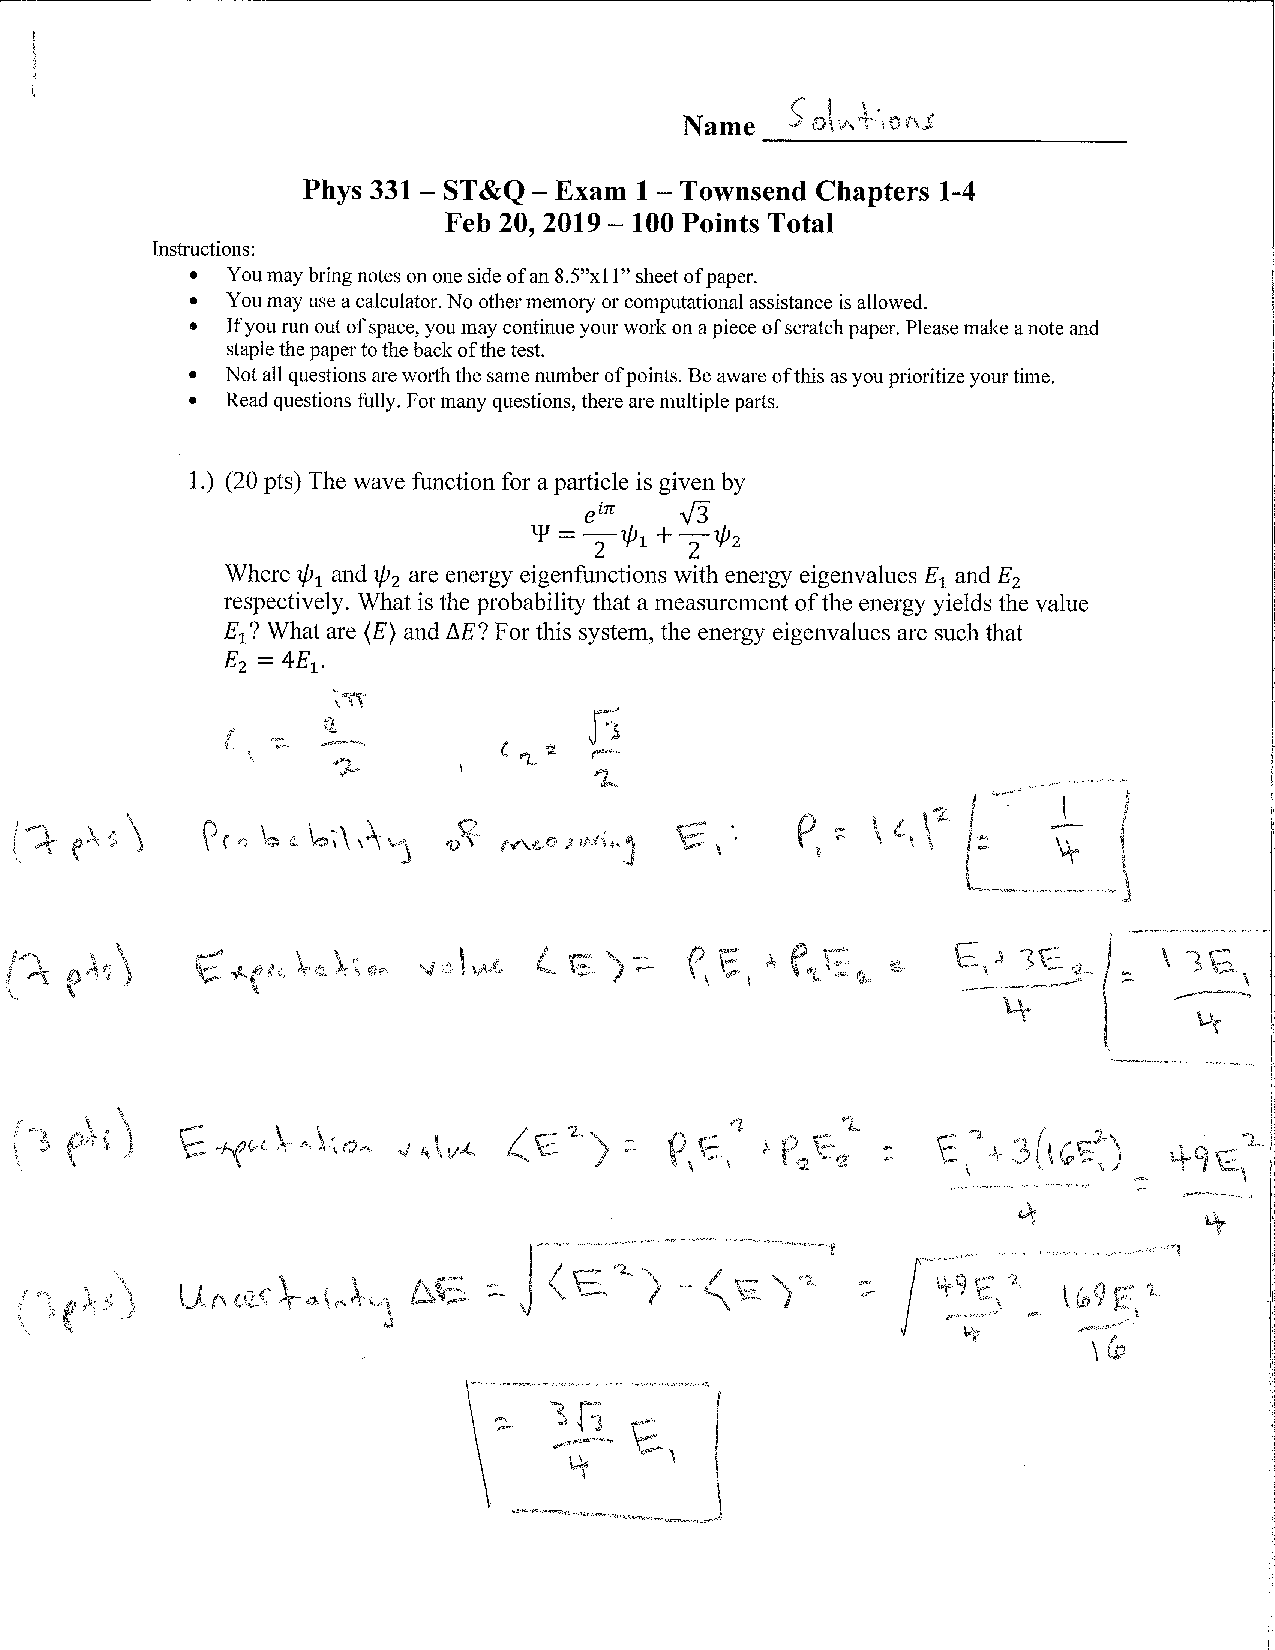
\includegraphics[scale=.31]{exam1.pdf}
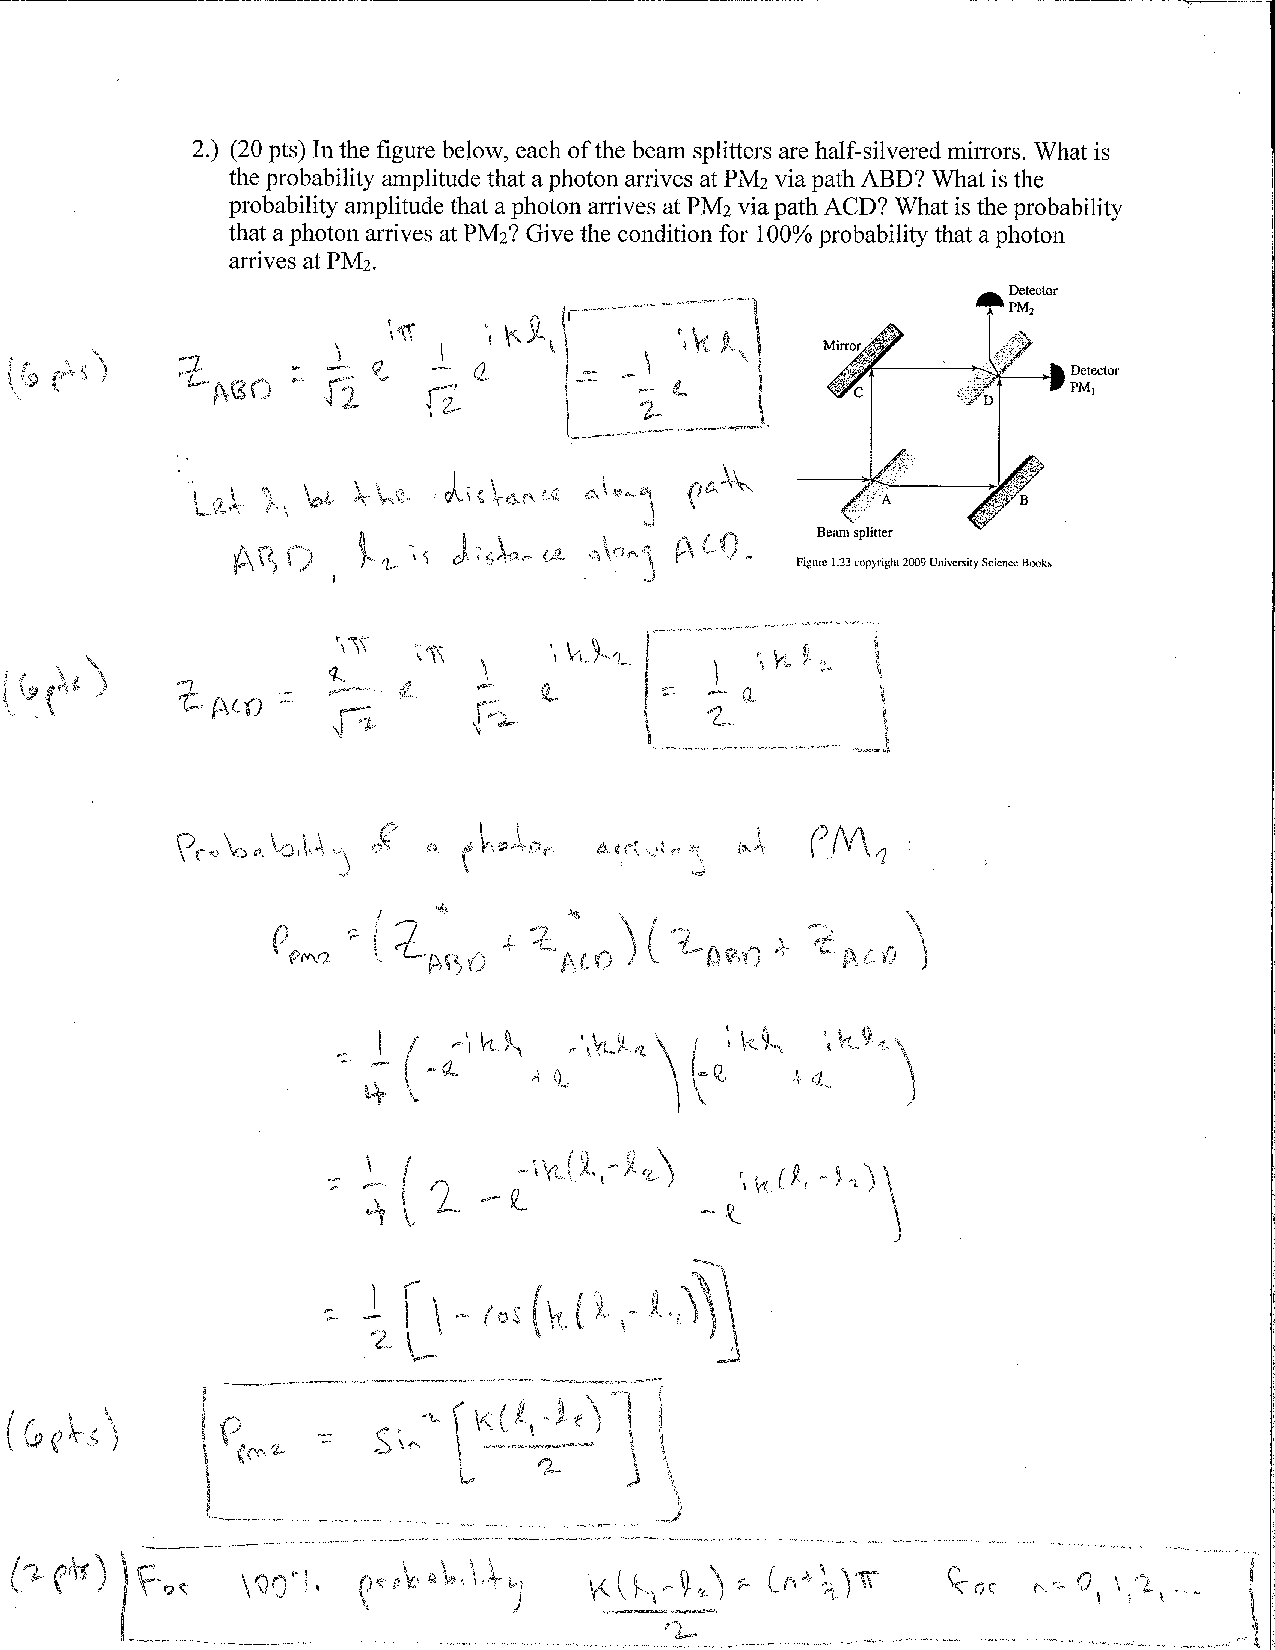
\includegraphics[scale=.31]{exam12.pdf}
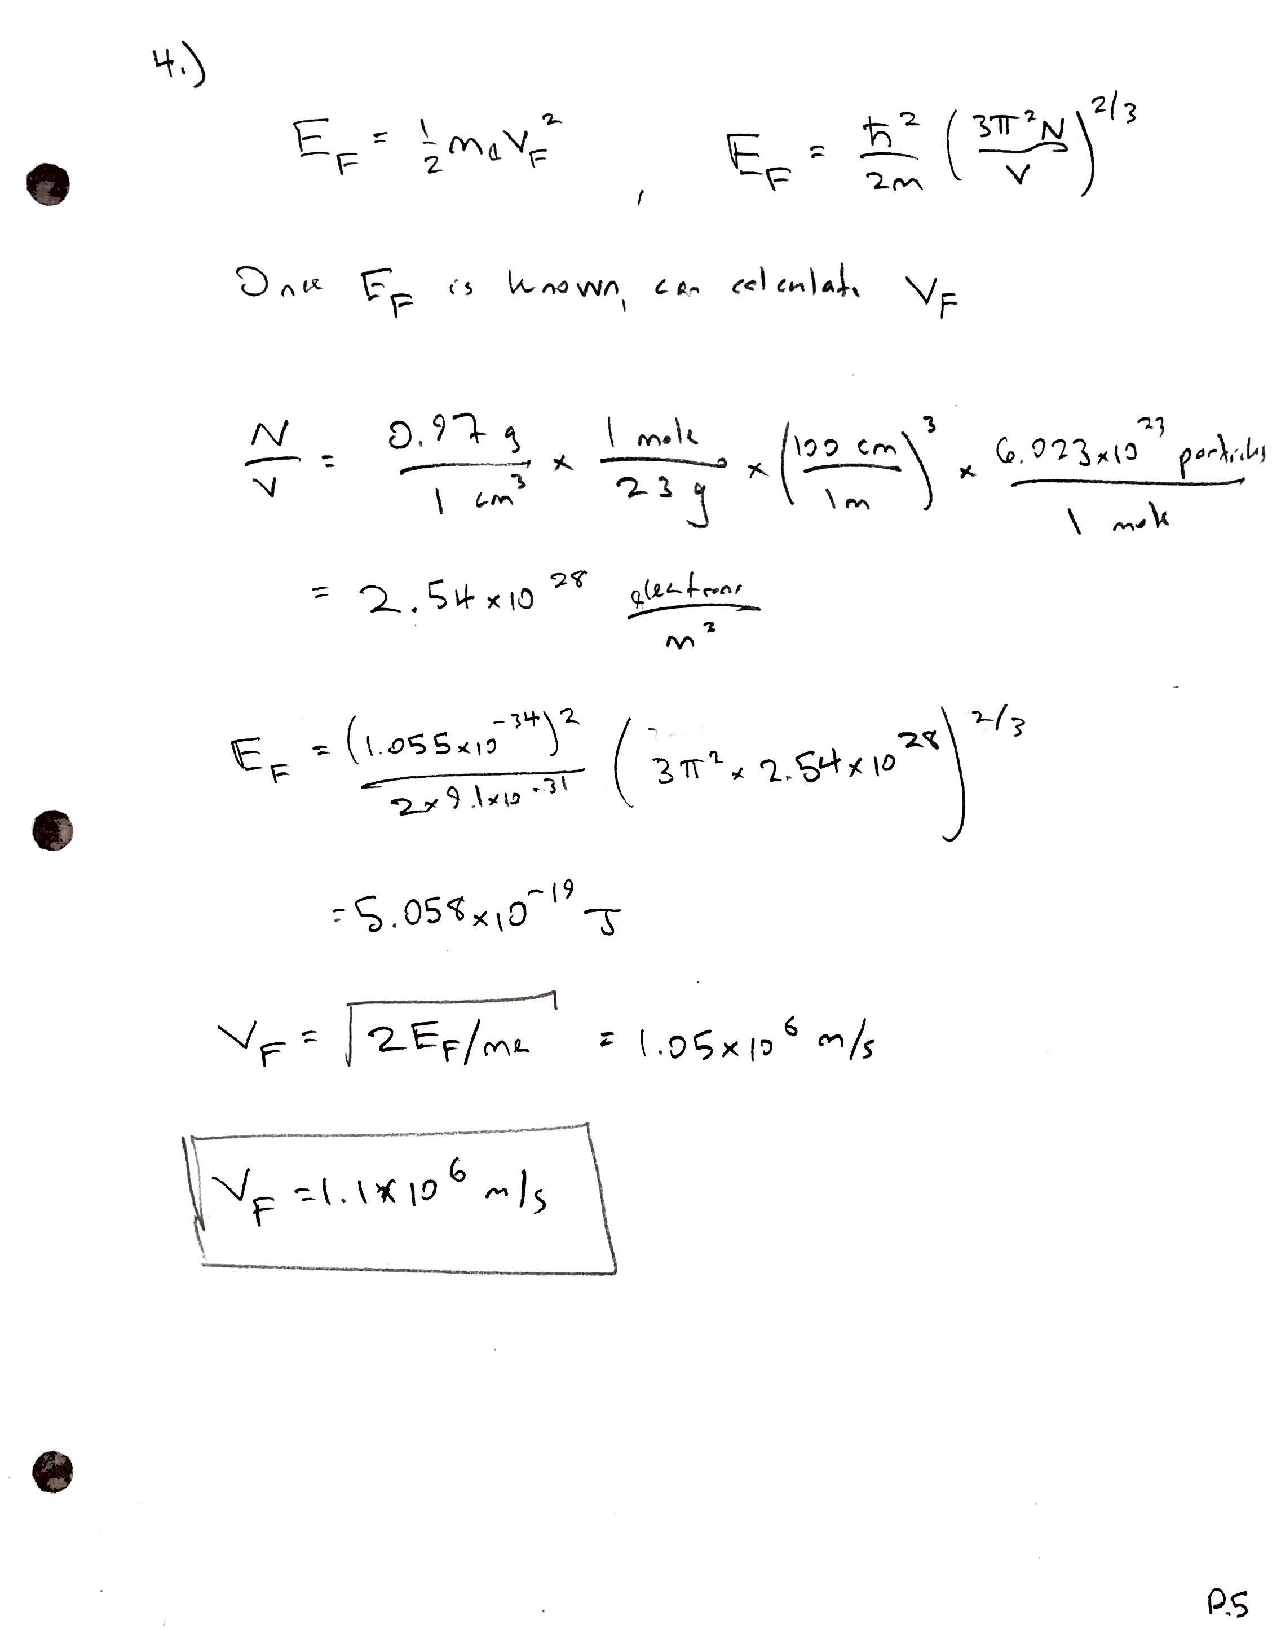
\includegraphics[scale=.31]{exam13.pdf}
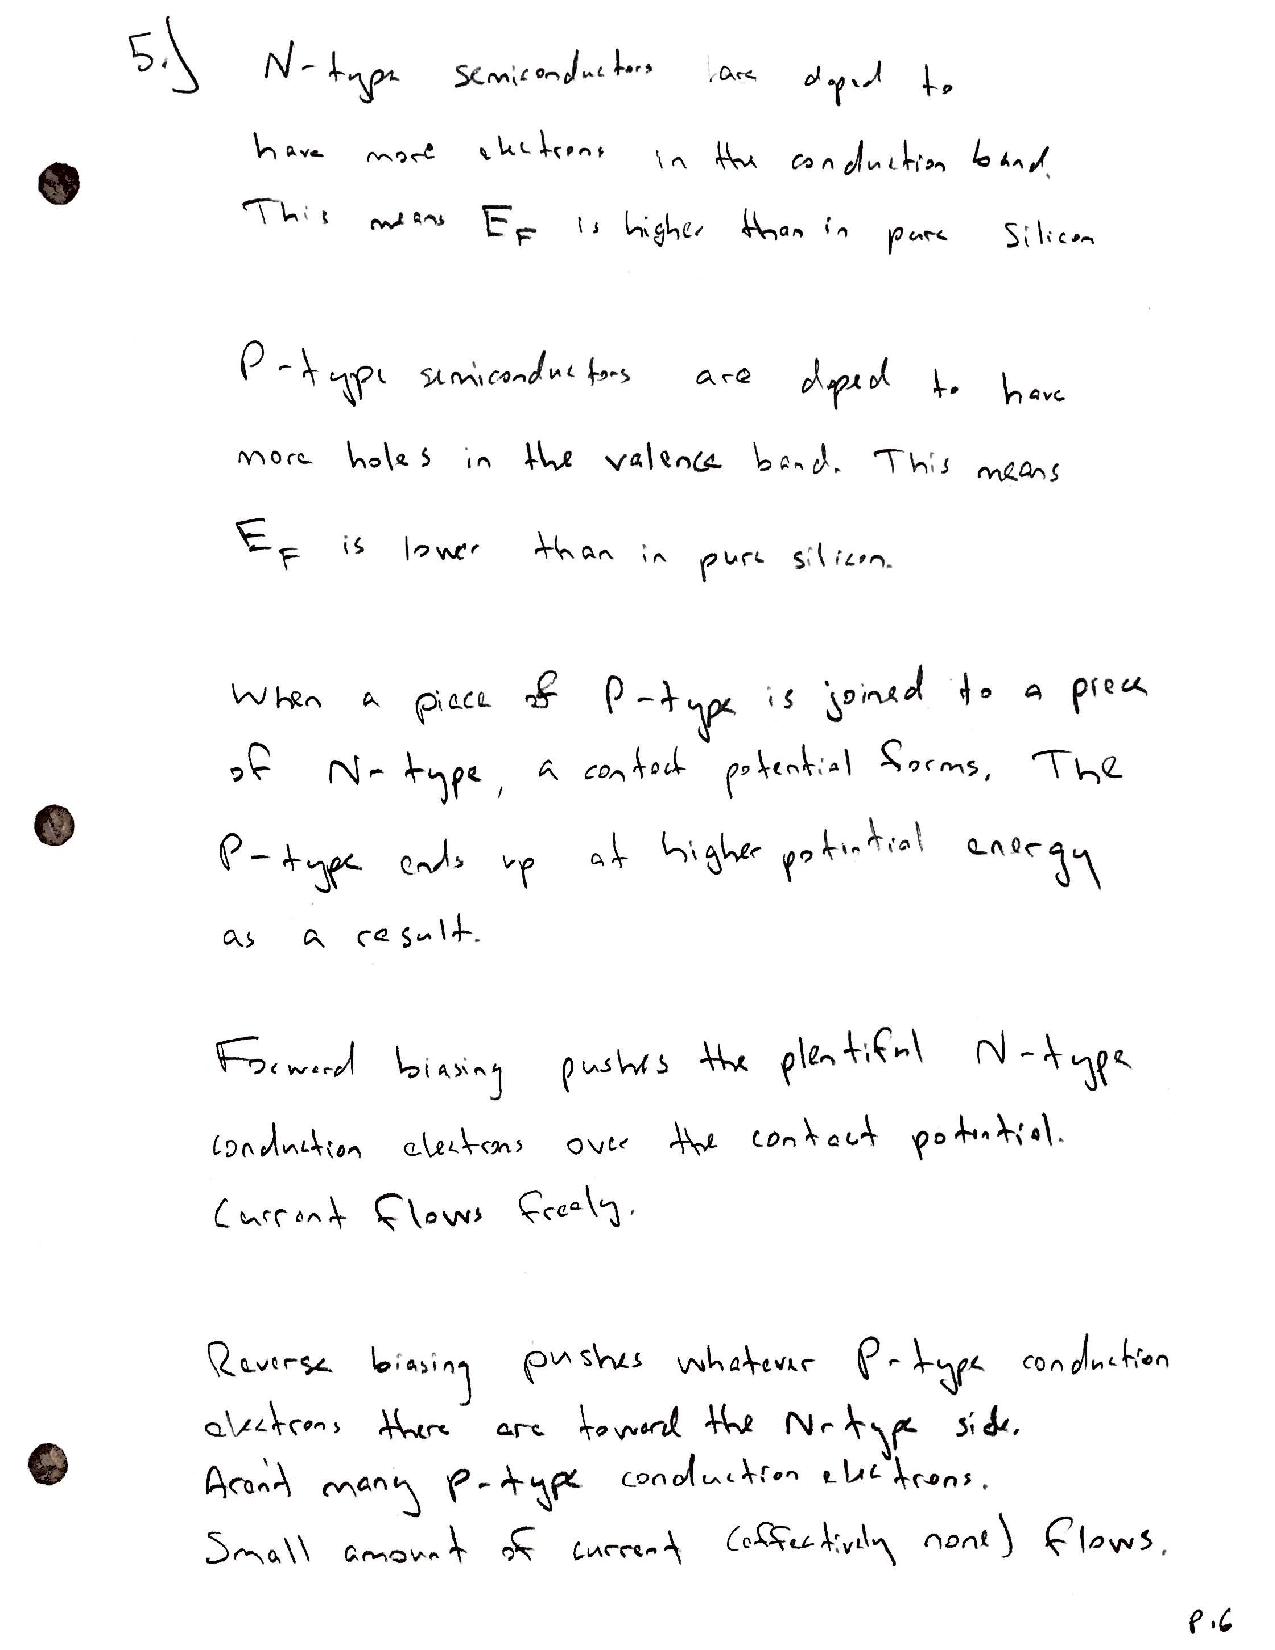
\includegraphics[scale=.31]{exam14.pdf}
\end{flushleft}
\end{multicols*}
\end{document}